\chapter{Visualizing Dynamic Input Graphs}
\label{chap:visualizing-dynamic-input-graphs}

Extending the approach discussed in the previous section to dynamic input graphs is challenging primarily because we must try to preserve the viewer's mental map as the underlying data changes over time. We want the visualization at different points in time to be similar enough so that the viewer can clearly tell what parts have changed \cite{mashima2011visualizing}, yet allow for the required changes in geography and topology. Still, changes between visualizations at consecutive points in time should minimize movement and allow for smooth animations therebetween.

The pipeline for static inputs discussed in the previous section does not satisfy these requirements. Running through the entire pipeline with a different, albeit similar, input graph, may result in a completely different visualization, destroying the viewer's mental map. We therefore extend the pipeline in a way that allows for small, incremental changes to be propagated through the pipeline and to eventually be applied to the previous output in a way that preserves the viewer's mental map.

We extend the pipeline for static input by an incremental transformation phase. This phase takes two inputs: A proportional map graph $G_\text{prop}$ that the pipeline previously produced as output for some cluster graph $G_\text{emb}$, and a sequence of operations on said cluster graph, that, when applied to $G_\text{emb}$, yields the cluster graph $G_\text{emb}^\prime$. The incremental embedding phase then determines how these operations translate to a polygonal dual of $G_\text{emb}$ and applies the translated operations to $G_\text{prop}$, producing $G_\text{init}^\prime$, a (not necessarily approximately area-proportional) polygonal dual of $G_\text{emb}^\prime$. This polygonal dual is then fed back into the drawing phase to make it approximately area-proportional and improve the local fatness of the map's regions.

\begin{figure}[H]
	\centering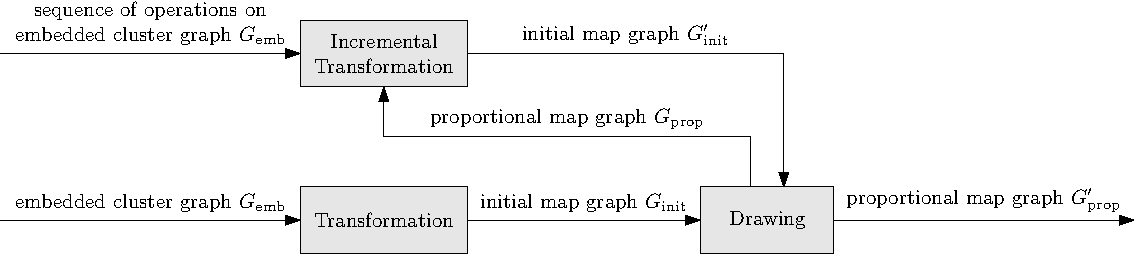
\includegraphics[width=0.9\textwidth]{Resources/Pipeline-Thesis-Dynamic.pdf}
	\caption{Overview of the algorithmic pipeline for dynamic input graphs.}
	\label{fig:dynamic-pipeline-thesis}
\end{figure}

Real-world applications such as visualizing a dynamic opinion network need a way to feed a sequence of operations on the embedded cluster graph into our framework. This could be done by prepending an incremental clustering phase that translates changes to the simple input graph into changes of its embedded cluster graph. However, such a sequence of operations is only meaningful in combination with a graph that these operations can be applied to. One must provide the previously-produced cluster graph as additional input to the incremental clustering phase such that it can tailor its output to the cluster graph that has already been locked in in an earlier run through the pipeline.

This tweak to our pipeline is illustrated in the following figure:
%
\begin{figure}[H]
	\centering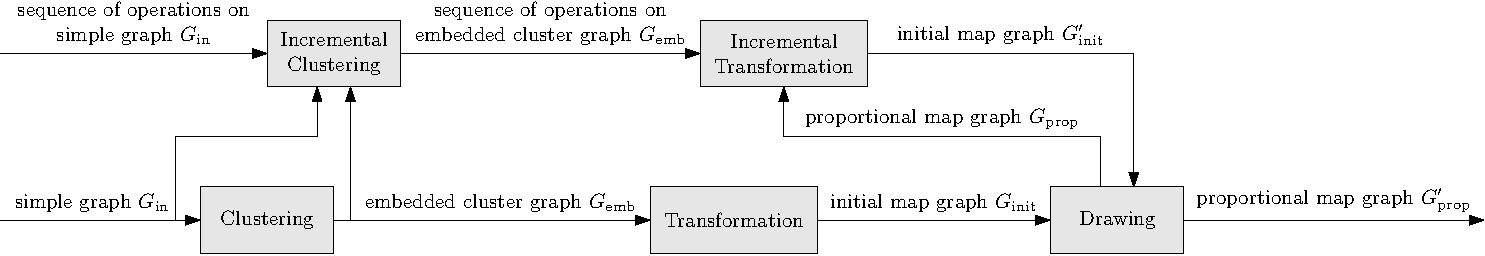
\includegraphics[width=0.9\textwidth]{Resources/Pipeline-Application-Dynamic.pdf}
	\caption{Overview of a possible algorithmic pipeline for generic applications.}
	\label{fig:dynamic-pipeline-application}
\end{figure}

Extending the pipeline to allow the propagation of small, incremental changes of the input graph has numerous benefits other than the ability to preserve the viewer's mental map:
%
\begin{itemize}
	\item It allows highly efficient implementations of the incremental parts of the pipeline as only the aspects that have actually changed in the input graph or intermediate products need to be processed and propagated further along the pipeline.
	\item It makes the dynamic pipeline highly parallelizable: when a later phase is processing changes, an earlier phase can already start processing new changes independently. With our force-directed implementation of the drawing phase, we can even incorporate dynamic updates while the drawing phase is still running, even if it has not converged yet: we pause the force simulation, feed the current map graph $G_\text{prop}$ into the incremental transformation phase to incorporate the dynamic updates, and then resume the simulation with the updated map graph $G_\text{init}^\prime$ produced by the incremental transformation phase.
	\item It efficiently supports dynamic input in an online setting, \ie{} a setting in which the incremental changes aren't known in advance, for example when visualizing live data.
\end{itemize}



\paragraph{Supported Operations}

Our pipeline supports numerous classes of primitive operations on the cluster graph, such as inserting and removing vertices and edges, flipping edges, or simply changing a cluster's weight. By composing multiple primitive operations in a sequence, more drastic changes can be made to the cluster graph. In our pipeline, the operations are applied one by one nonetheless.

The simplest operation of all is changing a vertex $v$'s weight: We simply take the previous proportional map graph $G_\text{prop}$, update the weight of the face $f_v$ corresponding to the vertex $v$, and declare that as the new initial map graph $G_\text{init}^\prime$. $G_\text{init}^\prime$ then runs through the drawing phase again to account for the updated face weights.

Implementing the remaining operations as part of the incremental transformation is a little more challenging, and we'll discuss those in great detail in the following sections.

\clearpage
\section{Inserting Vertices}
\label{sect:inserting-vertices}

When a new cluster appears in our underlying data set, we want to add a new vertex to the cluster graph. We distinguish between adding a new vertex on the inside and adding a new vertex on the outside because different rules apply.



\paragraph{Inserting Vertices Inside}

All internal faces of the cluster graph are triangles. If we add a vertex in one of the triangular faces, we must also add edges to the three vertices bounding the face without introducing edge crossings in order to preserve the graph's internal triangulatedness. A valid vertex insertion into an internal face is illustrated in \cref{fig:insert-vertex-inside-example}.

\begin{figure}[H]
	\centering
	\subfigure[]{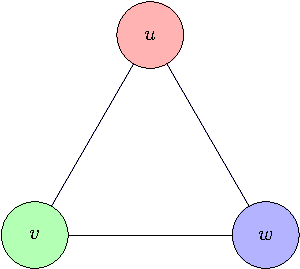
\includegraphics[height=29mm]{Resources/InsertVertexInside-Example-1.pdf}}
	\quad
	\subfigure[]{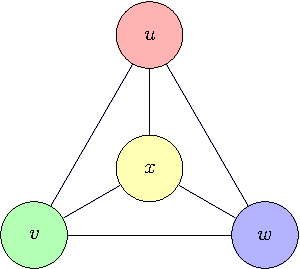
\includegraphics[height=29mm]{Resources/InsertVertexInside-Example-2.pdf}}
	\qquad
	\subfigure[]{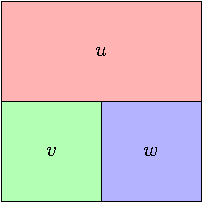
\includegraphics[height=29mm]{Resources/InsertVertexInside-Example-3.pdf}}
	\quad
	\subfigure[]{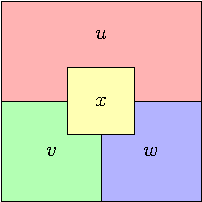
\includegraphics[height=29mm]{Resources/InsertVertexInside-Example-4.pdf}}
	\caption{A cluster graph and a polygonal dual thereof, before (a, c) and after (b, d) inserting the vertex $x$ in the triangular face $uvw$.}
	\label{fig:insert-vertex-inside-example}
\end{figure}

Let $u$, $v$, and $w$ be the vertices bounding an internal face of the cluster graph in counterclockwise order and $x$ the new vertex we want to add inside said face. We compute the paths that form the $u$-$v$-, $v$-$w$-, and $w$-$u$-boundaries in the polygonal dual. Let $p_{uvw}$ denote the vertex where the three faces corresponding to $u$, $v$, and $w$ meet. Let $p_{uv}$, $p_{vw}$, and $p_{wu}$ denote the first subdivision vertex on the boundary between faces $u$ and $v$, $v$ and $w$, and $w$ and $u$, respectively, starting from $p_{uwv}$. If one of the boundaries consist of only one edge, we place a subdivision vertex at its midpoint first. \Cref{subfig:insert-vertex-inside-illustration-1} shows how these vertices might look for the example from above.

\begin{figure}[H]
	\centering
	\subfigure[]{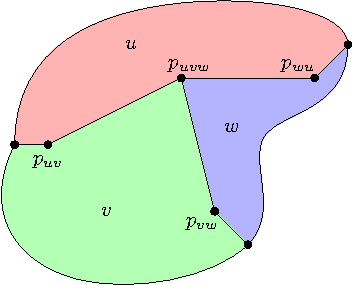
\includegraphics[width=45mm]{Resources/InsertVertexInside-Illustration-1.pdf}\label{subfig:insert-vertex-inside-illustration-1}}
	\quad
	\subfigure[]{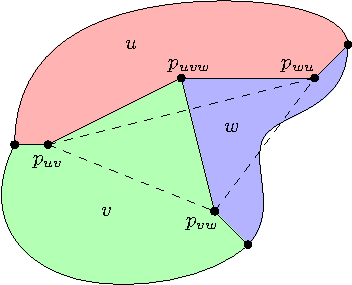
\includegraphics[width=45mm]{Resources/InsertVertexInside-Illustration-2.pdf}\label{subfig:insert-vertex-inside-illustration-2}}
	\quad
	\subfigure[]{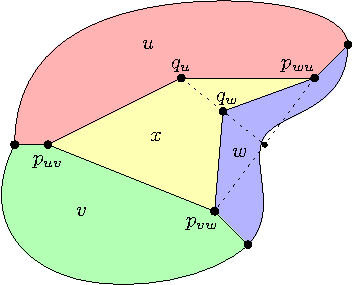
\includegraphics[width=45mm]{Resources/InsertVertexInside-Illustration-3.pdf}\label{subfig:insert-vertex-inside-illustration-3}}
	\caption{Inserting an internal face $x$ at the point where three faces $u,v,w$ meet.}
	\label{fig:insert-vertex-inside-illustration}
\end{figure}

Having determined the subdivision vertices $p_{uv}$, $p_{vw}$, and $p_{wu}$, we now want to remove the vertex $p_{uvw}$ and insert edges between the subdivision vertices instead to bound a new face for $d$ (dashed lines in \cref{subfig:insert-vertex-inside-illustration-2}). Doing so naïvely may introduce edge crossings and we generally need to add bends in the form of subdivision vertices to those edges. We distinguish three cases, all of which are illustrated in the figure:
%
\begin{itemize}
	\item If we can place an edge between $p_{ab}$ and $p_{bc}$ without introducing an edge crossing, we do not need to bend the edge (face $v$ in \cref{subfig:insert-vertex-inside-illustration-3}).
	\item Otherwise, if the internal angle of face $a$ at $p_{abc}$ is more than half a turn, we place the bend $q_a$ at $p_{abc}$ (face $u$ in \cref{subfig:insert-vertex-inside-illustration-3}).
	\item Otherwise we search for a bend location $q_a$ somewhere on the line segment from the midpoint of $p_{ab}$ and $p_{bc}$ to $p_{abc}$. We start at the midpoint of $p_{ab}$ and $p_{bc}$ and divide the remaining distance to $p_{abc}$ in half until we find a bend location for which the bent edge from $p_{ab}$ to $p_{bc}$ would not create edge crossings (face $w$ in \cref{subfig:insert-vertex-inside-illustration-3}).
\end{itemize}

Considering at most one angle at $p_{uvw}$ can be more than half a turn, we place at most one bend there. By removing the vertex $p_{uvw}$ and inserting the edges $\{p_{uv},p_{vw}\}$, $\{p_{vw},p_{wu}\}$, and $\{p_{wu},p_{uv}\}$, potentially with bends $p_v$, $p_w$, and $p_u$, we create an internal face for $x$.



\paragraph{Inserting Vertices Outside}

Alternatively, we can add a new vertex in the outer face of the cluster graph. Such a vertex must be connected to at least two vertices on the outer face to preserve the graph's 2-connectivity and its neighbors must form a path on the original boundary of the cluster graph in order not to create holes and thereby violate its internal triangulatedness.

We restrict ourselves to adding new vertices in the outer face that are made incident to exactly 2 neighboring vertices. Let $\{u,v\}$ be an edge on the outer face, then we support adding a new vertex $x$ in the outer face and connecting it to both $u$ and $v$. \Cref{fig:insert-vertex-outside-example} illustrates a valid vertex insertion into the outer face.

\begin{figure}[H]
	\centering
	\subfigure[]{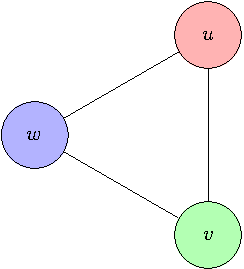
\includegraphics[height=29mm]{Resources/InsertVertexOutside-Example-1.pdf}}
	\quad
	\subfigure[]{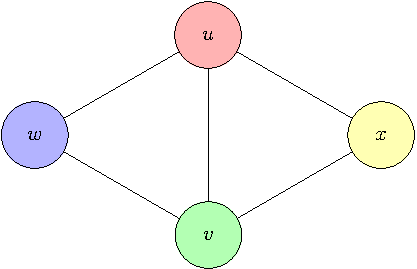
\includegraphics[height=29mm]{Resources/InsertVertexOutside-Example-2.pdf}}
	\qquad
	\subfigure[]{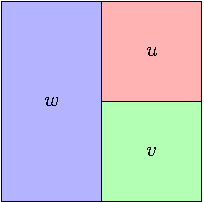
\includegraphics[height=29mm]{Resources/InsertVertexOutside-Example-3.pdf}}
	\quad
	\subfigure[]{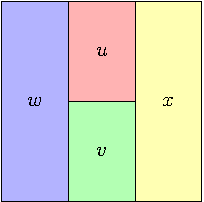
\includegraphics[height=29mm]{Resources/InsertVertexOutside-Example-4.pdf}}
	\caption{A cluster graph and a polygonal dual thereof, before (a, c) and after (b, d) inserting the vertex $x$ on the outer face and connecting it to $u$ and $v$.}
	\label{fig:insert-vertex-outside-example}
\end{figure}

Let $u$ and $v$ be the adjacent vertices on the outer face of the cluster graph and $x$ the new vertex we want to add in the outer face.
Let $p_{uv}$ denote the vertex where the faces $u$ and $v$ meet the outer face of the polygonal dual.
We define $p_u$ and $p_v$ as the first subdivision vertex we encounter when starting at $p_{uv}$ and following the boundary of $u$ and $v$ with the outer face, respectively.
If one of the boundaries consist of only one edge, we place a subdivision vertex at its midpoint and use that vertex as $p_u$/$p_v$.
\Cref{subfig:insert-vertex-outside-illustration-1} shows how these vertices might look for the example from above.
%

\begin{figure}[H]
	\centering
	\subfigure[]{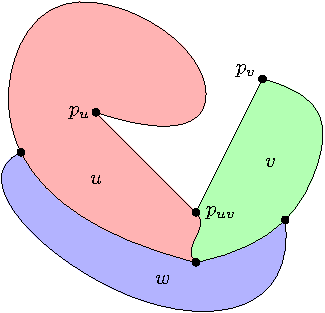
\includegraphics[width=45mm]{Resources/InsertVertexOutside-Illustration-1.pdf}\label{subfig:insert-vertex-outside-illustration-1}}
	\quad
	\subfigure[]{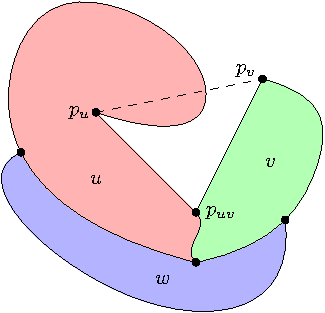
\includegraphics[width=45mm]{Resources/InsertVertexOutside-Illustration-2.pdf}\label{subfig:insert-vertex-outside-illustration-2}}
	\quad
	\subfigure[]{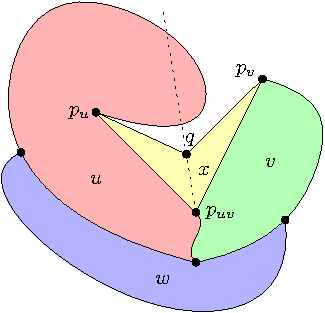
\includegraphics[width=45mm]{Resources/InsertVertexOutside-Illustration-3.pdf}\label{subfig:insert-vertex-outside-illustration-3}}
	\caption{Inserting a face $x$ at the point where the faces $u$ and $v$ meet the outer face.}
	\label{fig:insert-vertex-outside-illustration}
\end{figure}

With $p_u$ and $p_v$ determined, we can create the face $x$ by inserting a path to connect $p_u$ and $p_v$ without introducing edge crossings. Simply inserting an edge between $p_u$ and $p_v$ generally isn't enough, as illustrated in \cref{subfig:insert-vertex-outside-illustration-2}. However, with a single bend in the form of a subdivision vertex $q$, we can guarantee that no edge crossings are being created.

We search for a bend location on the outward-pointing bisector of the angle $\measuredangle_{p_up_{uv}p_v}$, starting at some fixed distance $\epsilon > 0$ and halving the distance until we find a valid location. As the possible bend location moves infinitesimally close to $p_{uv}$, we are guaranteed to find one that doesn't introduce edge crossings. By inserting a vertex at $q$ along with edges $\{q,p_u\}$ and $\{q,p_v\}$, we create an internal face for $x$, as illustrated in \cref{subfig:insert-vertex-outside-illustration-3}.

\clearpage
\section{Removing Vertices}
\label{sect:removing-vertices}

Clusters in the underlying data set can also fade and eventually cease to exist. In this case, we want to be able to remove existing vertices of the cluster graph. We make the same distinction here as when inserting vertices: we can remove internal vertices or vertices that lie on the cluster graph's outer face. 



\paragraph{Removing Internal Vertices}

When removing an internal vertex, we must ensure that the cluster graph remains internally triangulated. This is only the case if the vertex we want to remove has degree 3 as removing vertices with greater degree would create holes. If one wants to a vertex with degree 4 or higher, one must first tweak the adjacencies on the inside of the cluster graph using edge flips, discussed in \cref{sect:flipping-edges}. \Cref{fig:remove-vertex-example-internal} shows a valid removal of an internal vertex.

\begin{figure}[H]
	\centering
	\subfigure[]{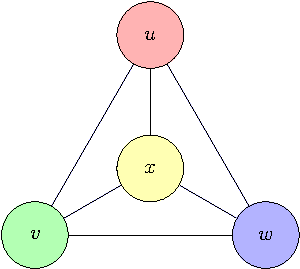
\includegraphics[height=29mm]{Resources/RemoveVertex-Example-Internal-1.pdf}}
	\quad
	\subfigure[]{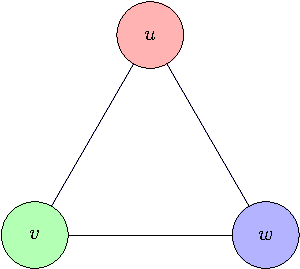
\includegraphics[height=29mm]{Resources/RemoveVertex-Example-Internal-2.pdf}}
	\qquad
	\subfigure[]{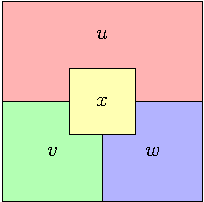
\includegraphics[height=29mm]{Resources/RemoveVertex-Example-Internal-3.pdf}}
	\quad
	\subfigure[]{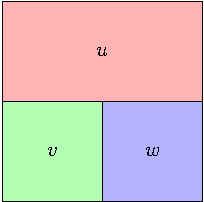
\includegraphics[height=29mm]{Resources/RemoveVertex-Example-Internal-4.pdf}}
	\caption{A cluster graph and a polygonal dual thereof, before (a, c) and after (d, d) removing the internal vertex $x$ with degree 3.}
	\label{fig:remove-vertex-example-internal}
\end{figure}

In order not to create holes in the contact representation, the incident faces must take over the area that the face to be removed originally occupied. Let $x$ denote the internal vertex we want to remove and $u$, $v$, and $w$ its three neighbors. We start by computing the paths that form the $u$-$v$-, $v$-$w$, and $w$-$u$-boundaries in the dual. Let $p_{uvx}$ ($p_{vwx}$, $p_{uwx}$) denote the vertex where face $x$ meets faces $u$ and $v$ ($v$ and $w$, $w$ and $u$). \Cref{subfig:remove-vertex-illustration-1} shows how these vertices might look for the example from above.

\begin{figure}[H]
	\centering
	\subfigure[]{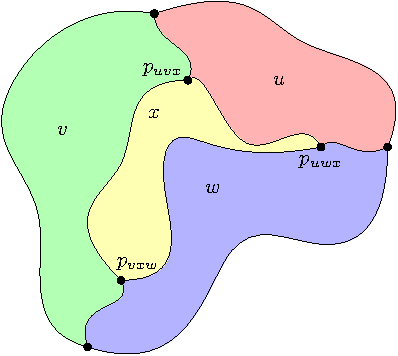
\includegraphics[width=45mm]{Resources/RemoveVertex-Illustration-1.pdf}\label{subfig:remove-vertex-illustration-1}}
	\quad
	\subfigure[]{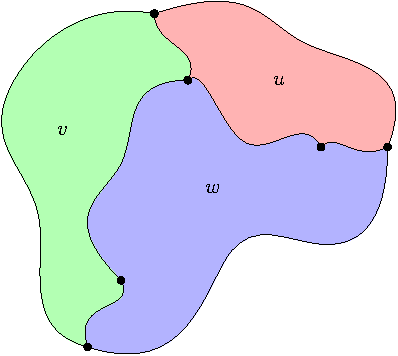
\includegraphics[width=45mm]{Resources/RemoveVertex-Illustration-2.pdf}\label{subfig:remove-vertex-illustration-2}}
	\caption{Removing an internal face $x$ incident to the faces $u$, $v$, and $w$.}
	\label{fig:remove-vertex-illustration}
\end{figure}

To remove the internal face $x$, we simply remove the its boundary to one of its neighboring faces. In doing so, the two faces effectively merge. In practice this works really well because large clusters don't disappear at a moment's notice, and small clusters generally occupy a very small area such that the operation is barely noticeable.




\paragraph{Removing External Vertices}

When removing vertices on the outer face along with its incident edges, we must ensure that the graph remains 2-connected afterwards. \cref{fig:remove-vertex-example-external} illustrates a valid removal of a vertex on the outer face. Similar to inserting vertices on the outer face, we restrict ourselves to removing vertices on the outer face that have degree 2. If we need to remove a vertex with higher degree, the additional edges need to be removed first as discussed in \cref{sect:flipping-edges}.

\begin{figure}[H]
	\centering
	\subfigure[]{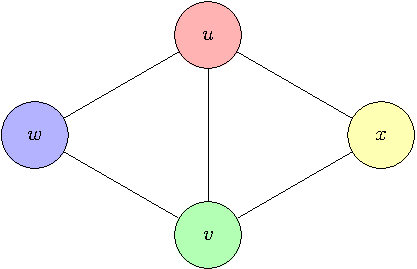
\includegraphics[height=29mm]{Resources/RemoveVertex-Example-External-1.pdf}}
	\quad
	\subfigure[]{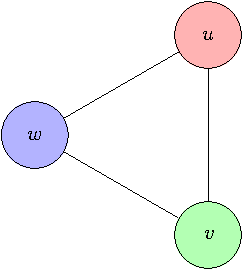
\includegraphics[height=29mm]{Resources/RemoveVertex-Example-External-2.pdf}}
	\qquad
	\subfigure[]{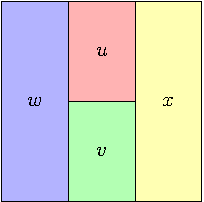
\includegraphics[height=29mm]{Resources/RemoveVertex-Example-External-3.pdf}}
	\quad
	\subfigure[]{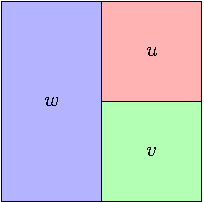
\includegraphics[height=29mm]{Resources/RemoveVertex-Example-External-4.pdf}}
	\caption{A cluster graph and a polygonal dual thereof, before (a, c) and after (b, d) removing the vertex $x$ on the outer face.}
	\label{fig:remove-vertex-example-external}
\end{figure}

This operation, too, is just a special case of the vertex removal discussed above. Referring to the construction of the augmented dual again, with the helper vertex $v^+$ and edges $\{v^+,\cdot\}$, removable vertices $x$ on the outer face of the cluster graph lie in a triangle formed by its two neighbors $u$ and $v$ and the helper vertex $v^+$.

The construction outlined above translates 1-to-1 to removing vertices from the outer face, except one of the three neighboring faces is the implicit outer face. In our implementation, we always remove the boundary of $x$ with the outer face and thereby transfer the area to the outer face.

\clearpage
\section{Inserting Edges}
\label{sect:inserting-edges}

As clusters in our data set grow increasingly similar, we may want to indicate this similarity with a new edge between two clusters in the cluster graph. However, because the cluster graph is internally triangulated, we cannot insert any more edges on the inside of the graph. We can only insert edges in the outer face. Inserting an edge in the outer face is also only possible if it preserves the internal triangulatedness of the cluster graph. Inserting an edge $\{u,w\}$ in the outer face is therefore only permitted if $u$ and $w$ have a neighbor $v$ in common such that adding the edge forms a new triangular face with $v$. A valid edge insertion is illustrated in \cref{fig:insert-edge-outside-example}.

\textbf{Insert edge on outer face:} Edges between nonadjacent vertices $u, v$ on the outer face may only be inserted if they preserve the graph's internal triangulatedness, \ie{} they don't create holes in the graph. Adding such an edge creates a new internal face and is therefore only possible iff $u$ and $v$ have a neighbor in common.

\begin{figure}[H]
	\centering
	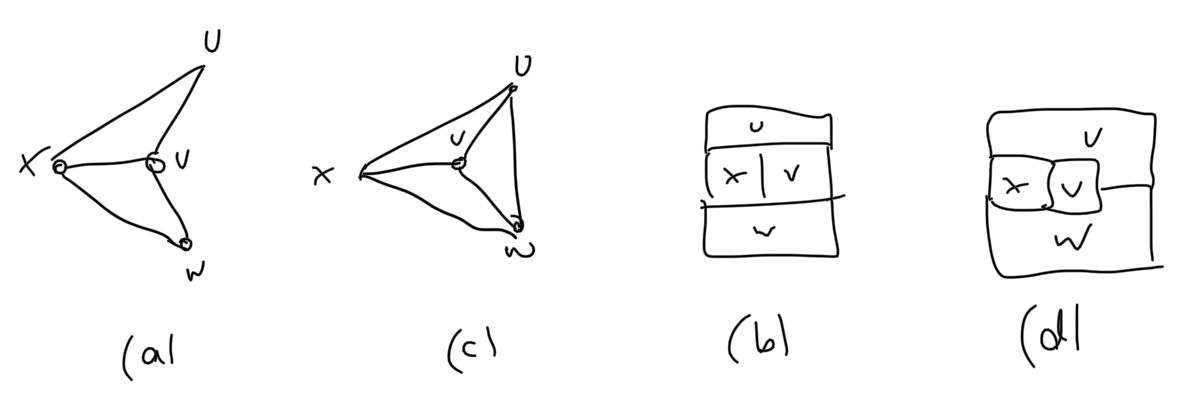
\includegraphics[height=30mm]{Resources/InsertEdgeOutside.png}
	\caption{A cluster graph and a polygonal dual thereof, before (a, b) and after (c, d) inserting the edge $\{u,w\}$ to form a triangular face with $v$.}
	\label{fig:insert-edge-outside-example}
\end{figure}

\clearpage
\section{Removing Edges}
\label{sect:removing-edges}

Similarly, clusters can grow apart and we may want to remove edges between clusters in the cluster graph.
This, too, is not allowed on the inside of the graph, as doing so would create holes and violate the graph's internal triangulatedness. We can only remove edges that lie on the outer face of the cluster graph. Even then, we must ensure that the graph remains $2$-connected. Removing an edge $\{u,w\}$ on the outer face is therefore only permitted if both $u$ and $w$ have degree $d(\cdot) \geq 3$. \cref{fig:remove-outer-edge-example} illustrates a valid edge removal.

\begin{figure}[H]
	\centering
	\subfigure[]{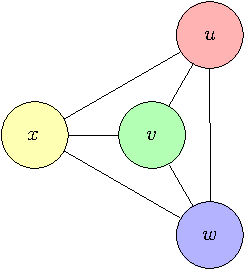
\includegraphics[height=29mm]{Resources/RemoveOuterEdge-Example-1.pdf}}
	\quad
	\subfigure[]{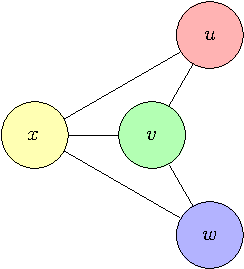
\includegraphics[height=29mm]{Resources/RemoveOuterEdge-Example-2.pdf}}
	\qquad
	\subfigure[]{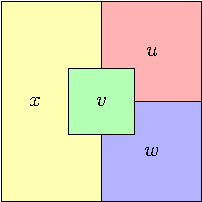
\includegraphics[height=29mm]{Resources/RemoveOuterEdge-Example-3.pdf}}
	\quad
	\subfigure[]{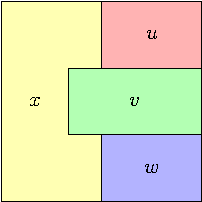
\includegraphics[height=29mm]{Resources/RemoveOuterEdge-Example-4.pdf}}
	\caption{A cluster graph and a polygonal dual thereof, before (a, b) and after (c, d) removing the edge $\{u,w\}$.}
	\label{fig:remove-outer-edge-example}
\end{figure}

\lipsum

\clearpage
\section{Flipping Edges}
\label{sect:fliping-edges}

Let us now look at operations involving only edges. We cannot add new edges inside, because the cluster graph is already internally triangulated. And we can't remove internal edges either, because that would create a hole and violate the internal triangulatedness. However, we can flip internal edges:

An internal edge $\{u,v\}$ is incident to two different internal faces $f$, $g$. Let $x$ and $y$ denote the third vertex bounding $f$ and $g$, respectively. It is $x \neq y$ because the cluster graph is simple. Flipping the edge $\{u,v\}$ would replace it with the edge $\{x,y\}$. This operation is therefore only permitted if $x$ and $y$ are not already adjacent \emdash{} otherwise we would introduce a duplicate adjacency. A valid edge flip operation is illustrated in \cref{fig:flip-internal-edge-example}.

\begin{figure}[H]
	\centering
	\subfigure[]{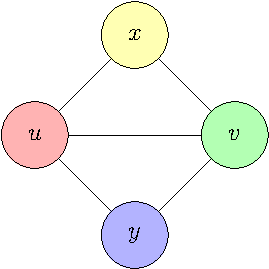
\includegraphics[width=30mm]{Resources/FlipInternalEdge-Example-1.pdf}}
	\quad
	\subfigure[]{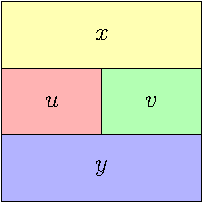
\includegraphics[width=30mm]{Resources/FlipInternalEdge-Example-2.pdf}}
	\quad
	\subfigure[]{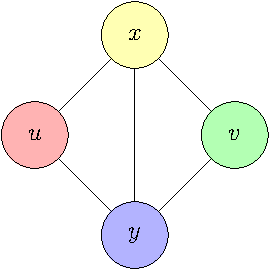
\includegraphics[width=30mm]{Resources/FlipInternalEdge-Example-3.pdf}}
	\quad
	\subfigure[]{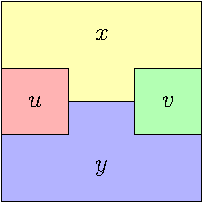
\includegraphics[width=30mm]{Resources/FlipInternalEdge-Example-4.pdf}}
	\caption{A cluster graph and a polygonal dual thereof, before (a, b) and after (c, d) flipping the internal edge $\{u,v\}$.}
	\label{fig:flip-internal-edge-example}
\end{figure}

An edge flip in a cluster graph translates to region adjacencies being flipped in its dual. Given a polygonal dual of some cluster graph, we apply an edge flip in two phases: First, we contract the respective region boundary into a single point, creating a degenerate contact representation in which 4 regions meet in a point. In the second phase, we create a new boundary in the opposite direction around that point the original boundary has been contracted into.

We contract a region boundary by repeatedly removing a peripheral edge of the boundary on alternating ends until the last edge of the boundary has been removed. To remove a peripheral edge of a boundary, let us consider the general case illustrated in \cref{fig:flip-internal-edge-contract}. We want to get rid of the edge $\{p_1,p_2\}$ on the red-green boundary. To do so, we  remove $p_2$ and its incident edges and add the new edges $\{p_3,p_1\}$ and $\{p_4,p_1\}$. This may introduce edge crossings though, as illustrated in \cref{subfig:flip-internal-edge-contract-crossing}. We may therefore need to introduce a bend to both new edges in the form of a subdivision vertex. We look for possible bend locations on the segment from $p_2$ to $p_3$ and $p_2$ to $p_4$, respectively, using binary search: We start at the far end, and cut the remaining distance to $p_2$ in half until we find a bend location that doesn't introduce edge crossings. As the distance from $p_2$ grows infinitesimally small, we are guaranteed to find a valid bend location.

\begin{figure}[H]
	\centering
	\subfigure[]{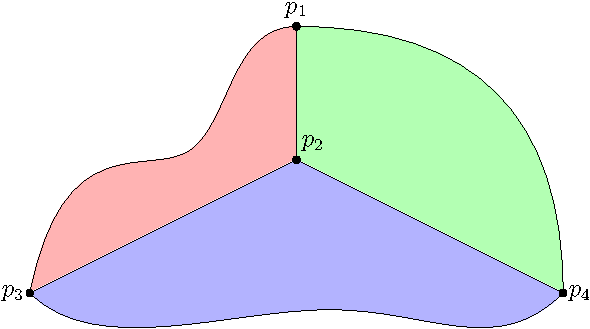
\includegraphics[width=40mm]{Resources/FlipInternalEdge-Contract-1.pdf}}
	\quad
	\subfigure[]{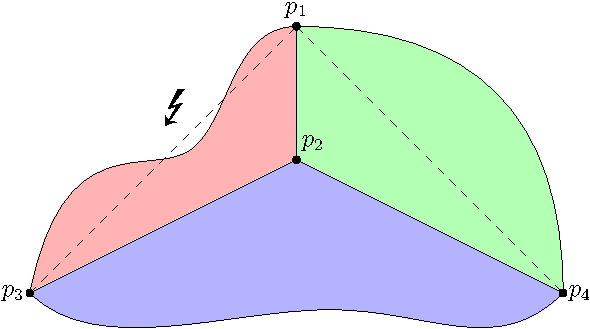
\includegraphics[width=40mm]{Resources/FlipInternalEdge-Contract-2.pdf}\label{subfig:flip-internal-edge-contract-crossing}}
	\quad
	\subfigure[]{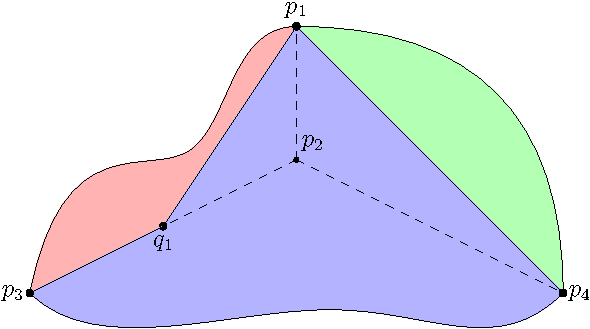
\includegraphics[width=40mm]{Resources/FlipInternalEdge-Contract-3.pdf}}
	\caption{A contact representation before (a) and after (c) removing the peripheral edge $\{p_1,p_2\}$ from the red-green boundary. (b) shows that we require a subdivision vertex $q_1$ on the red-blue boundary.}
	\label{fig:flip-internal-edge-contract}
\end{figure}

Once the boundary has been contracted into a single point, we need to resolve the degeneracy and create a boundary in the opposite direction as illustrated in \cref{fig:flip-internal-edge-expand}. If $\measuredangle_{p_1p_3p_4} < 180^\circ$, we search for a position in the face bounded by $p_1$, $p_3$, and $p_4$ at which we can place a new vertex $q_1$ and connect it to those three vertices without introducing edge crossings. We do this using another binary search on the segment from $p_3$ to the midpoint of $p_1$ and $p_4$. Once we found a valid position for $q_1$ and have added it to the graph along with the aforementioned edges, we remove the edges $\{p_3,p_1\}$ and $\{p_3,p_4\}$. We repeat the same for the face on the opposite side. Considering it is impossible for the angles to be more than half a turn on both sides, we have replaced at least one set of edges and have therefore successfully resolved the degeneracy and flipped the region adjacency.

\begin{figure}[H]
	\centering
	\subfigure[]{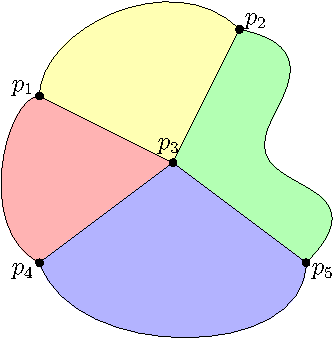
\includegraphics[width=30mm]{Resources/FlipInternalEdge-Expand-1.pdf}}
	\quad
	\subfigure[]{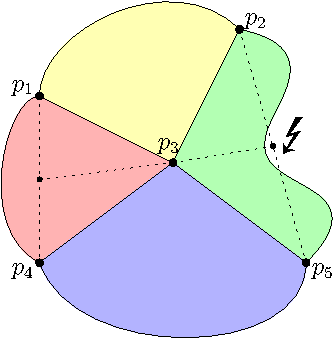
\includegraphics[width=30mm]{Resources/FlipInternalEdge-Expand-2.pdf}}
	\quad
	\subfigure[]{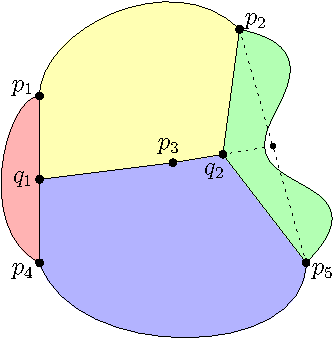
\includegraphics[width=30mm]{Resources/FlipInternalEdge-Expand-3.pdf}}
	\caption{A contact representation before (a) and after (c) creating a non-degenerate yellow-blue adjacency. (b) shows that $q_2$ cannot be the midpoint of $p_2$ and $p_5$ and needs to move further towards $p_3$.}
	\label{fig:flip-internal-edge-expand}
\end{figure}

